\section{Glossary}
\label{sec:glossary}

\begin{description}\itemsep0pt
\item[$\kappa$] per-track multiplier of the transverse momentum from the look-up table, $\pt^{\rm corr}=\kappa\pt$.
\item[$a$, $b$, $s$] curvature term, multiple-scattering term and global scale of the momentum response, Eq.~\ref{eq:model}.
\item[period A / B] runs 79509--79516 (range of the table) / all other runs of the sample.
\item[KFP / no $\kappa$ / with $\kappa$] the three mass versions: KFParticle fitted mass; recomputed from the stored daughter
  momenta; recomputed after the correction.
\item[DDSim] data-driven fast simulation of two-body V0 decays (DataDrivenSim project).
\item[DIRA] cosine of the angle between the V0 momentum and the PV-to-SV flight direction.
\item[DCA$_{12}$, DCA$_{xy}$] distance of closest approach between the daughters; transverse DCA of a daughter to the PV.
\item[$L_{xy}$] transverse decay length (PV to SV).
\item[QA cuts] offline V0 selection of Table~\ref{tab:sel}.
\item[tight \La{} selection] QA + DIRA$>$0.9995, $|{\rm DCA}_{xy}(\pi)|>0.10$, $|{\rm DCA}_{xy}(p)|>0.03$~cm (Sec.~\ref{sec:tight}).
\item[Baker--Cousins $\chi^2$] $2\sum_i[\mu_i-d_i+d_i\ln(d_i/\mu_i)]$, the Poisson likelihood-ratio goodness of fit.
\item[segment] one DST file of a run, about 990 events.
\end{description}

\appendix
\section{Template fits without the correction}
\label{app:raw}

\begin{figure}[H]
\centering
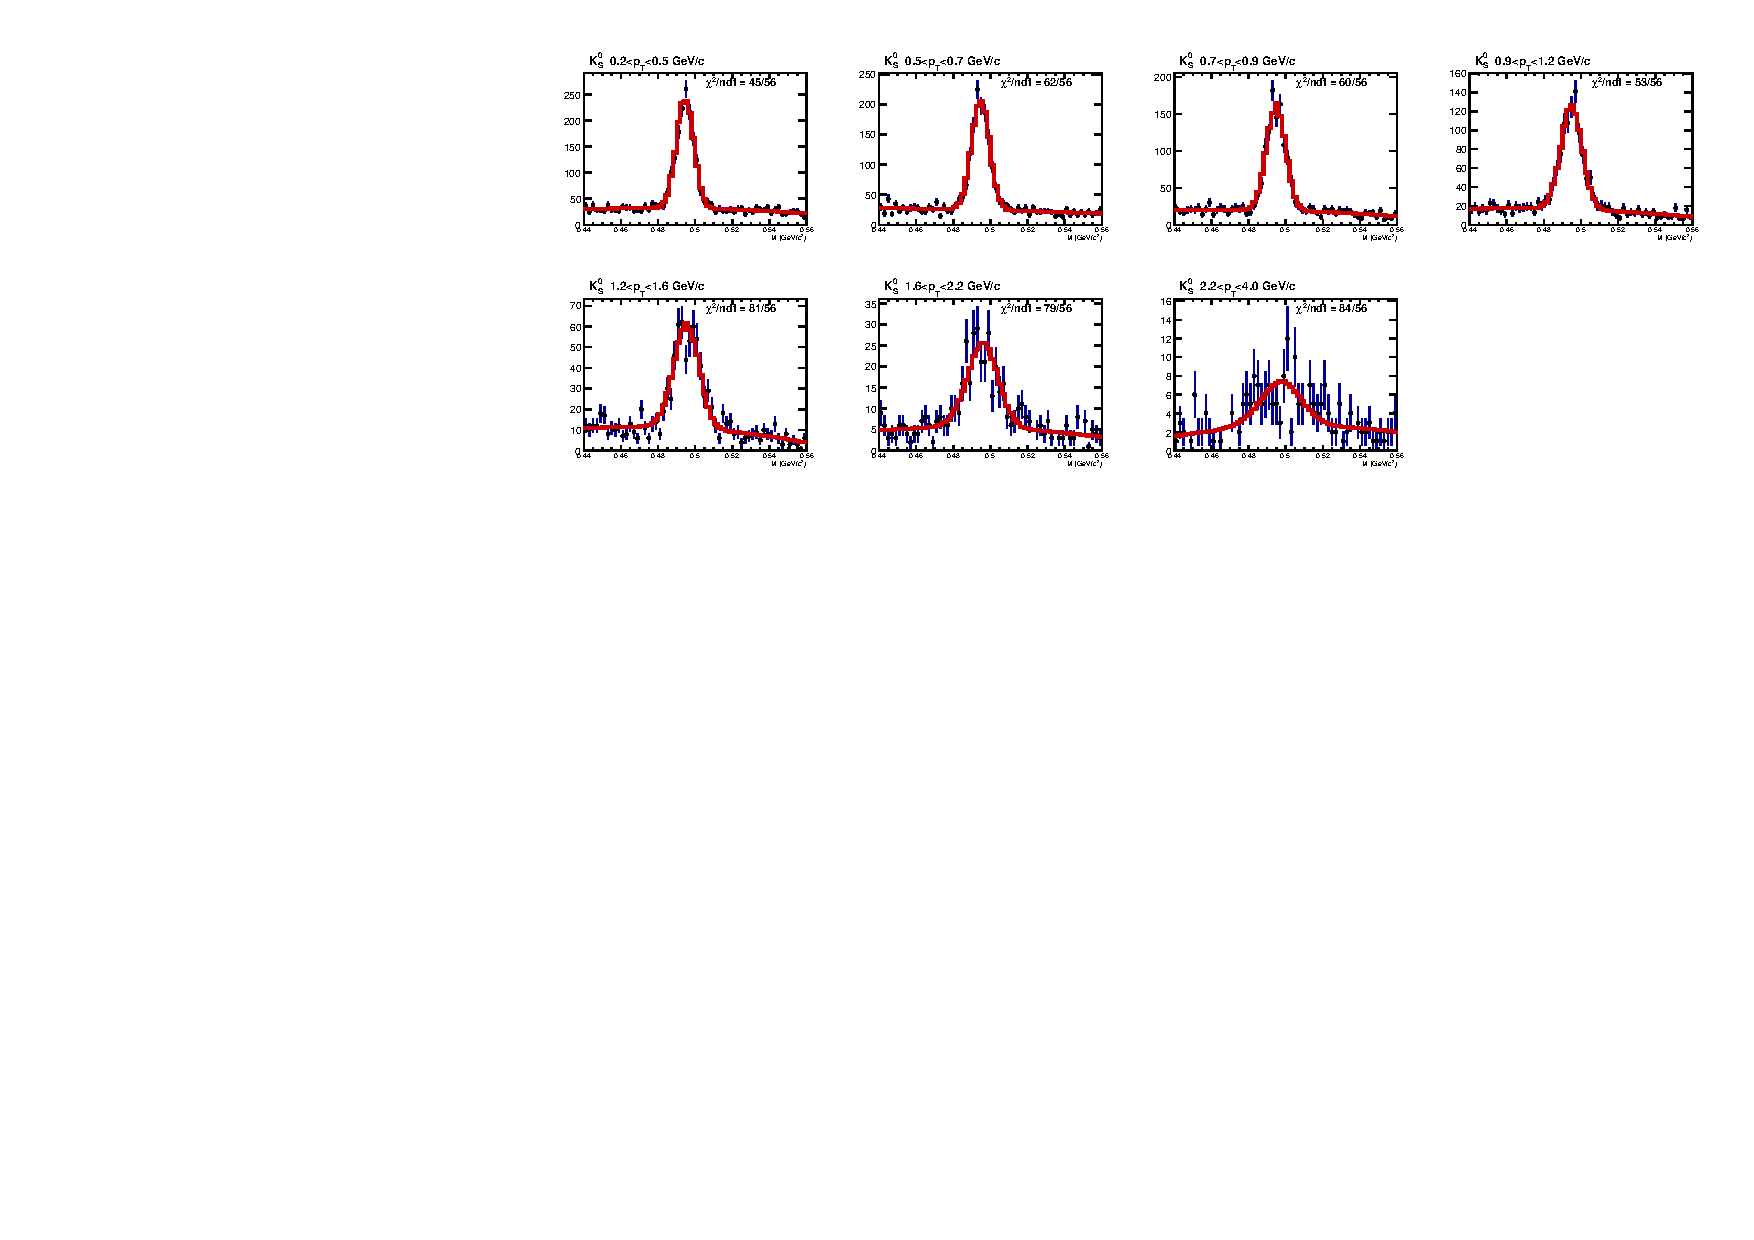
\includegraphics[width=\textwidth]{fig_mass_Ks_A_raw}
\caption{\Ks{} mass per V0-\pt{} bin, period A, recomputed without $\kappa$, with the template fit at that fit's \Ks{} best
point (red).}
\end{figure}

\begin{figure}[H]
\centering
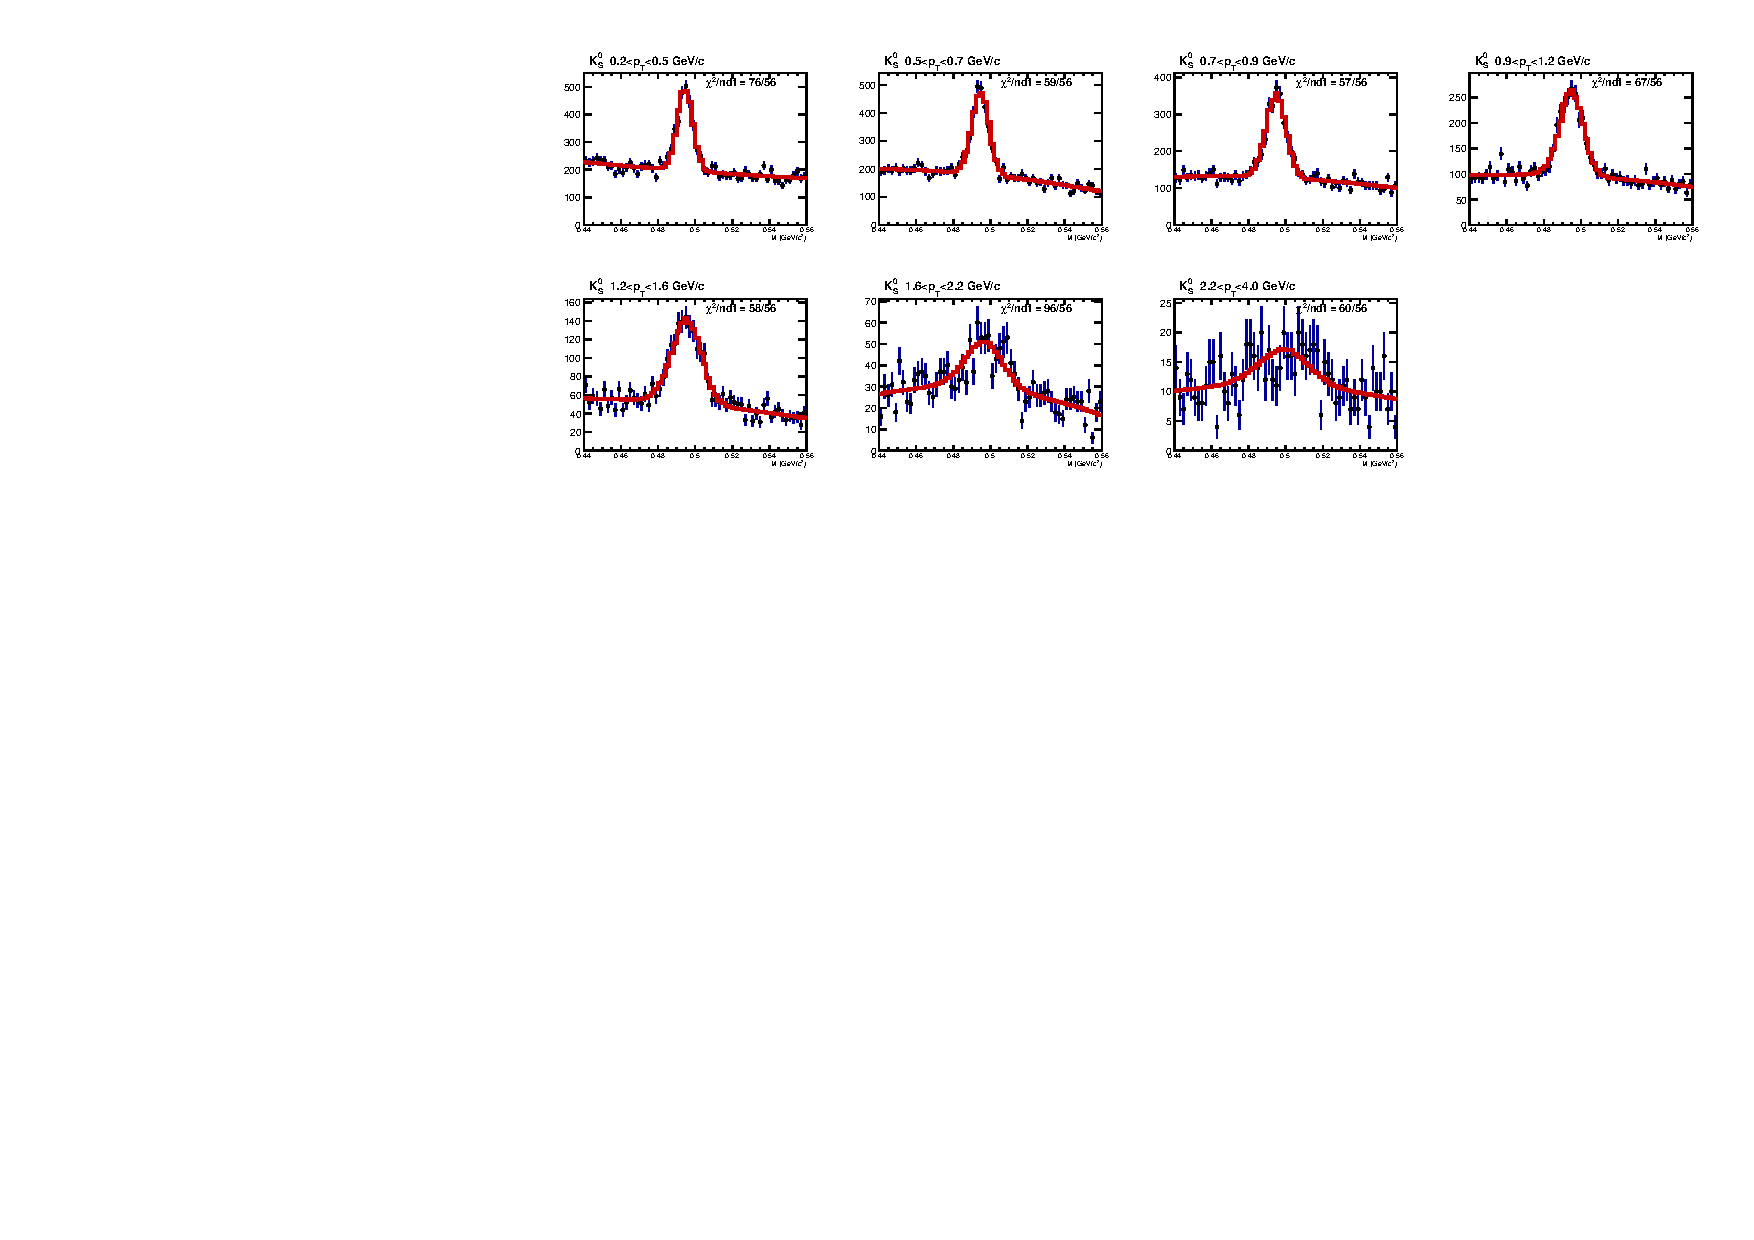
\includegraphics[width=\textwidth]{fig_mass_Ks_B_raw}
\caption{As above, period B.}
\end{figure}

\begin{figure}[H]
\centering
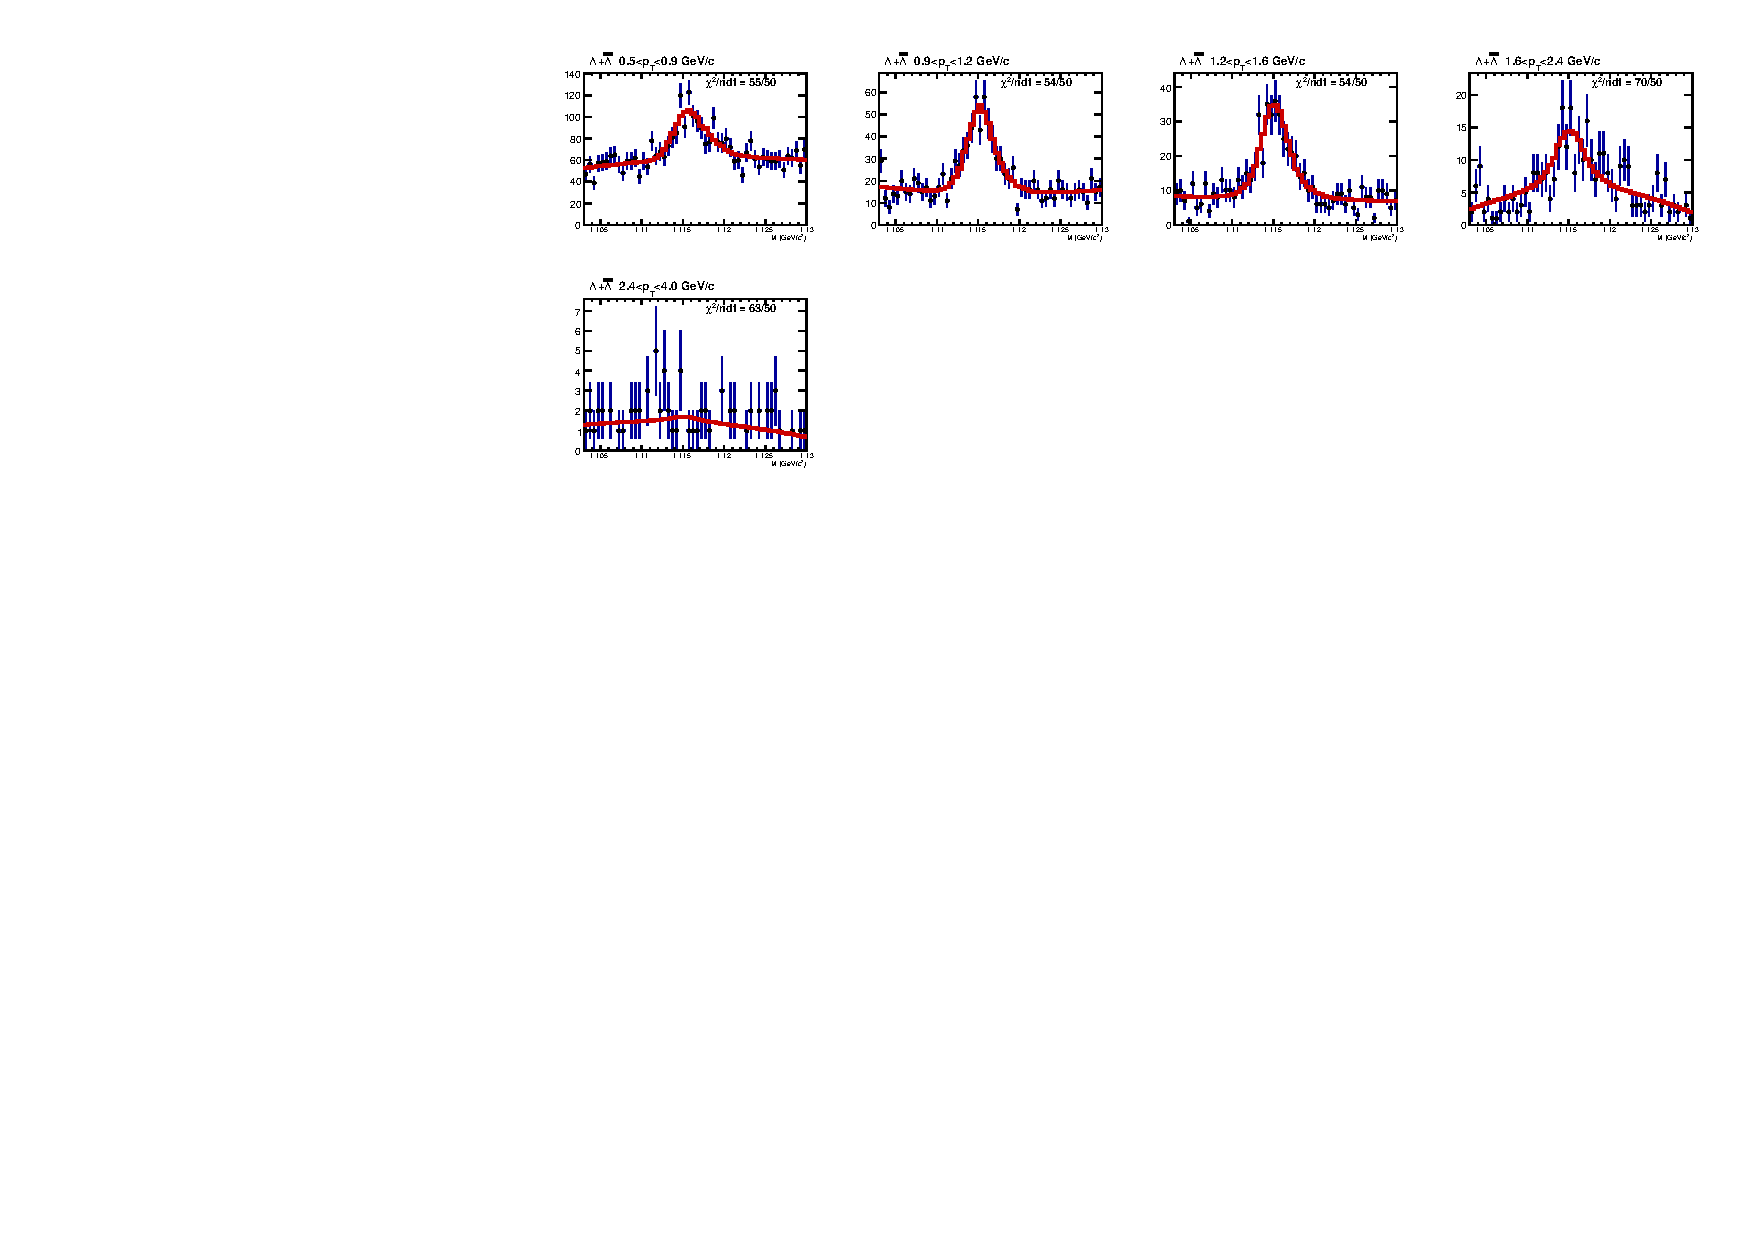
\includegraphics[width=\textwidth]{fig_mass_Lambda_A_raw}
\caption{\La+$\bar\Lambda$, period A, without $\kappa$; template at the \Ks{} best point of the same fit.}
\end{figure}

\begin{figure}[H]
\centering
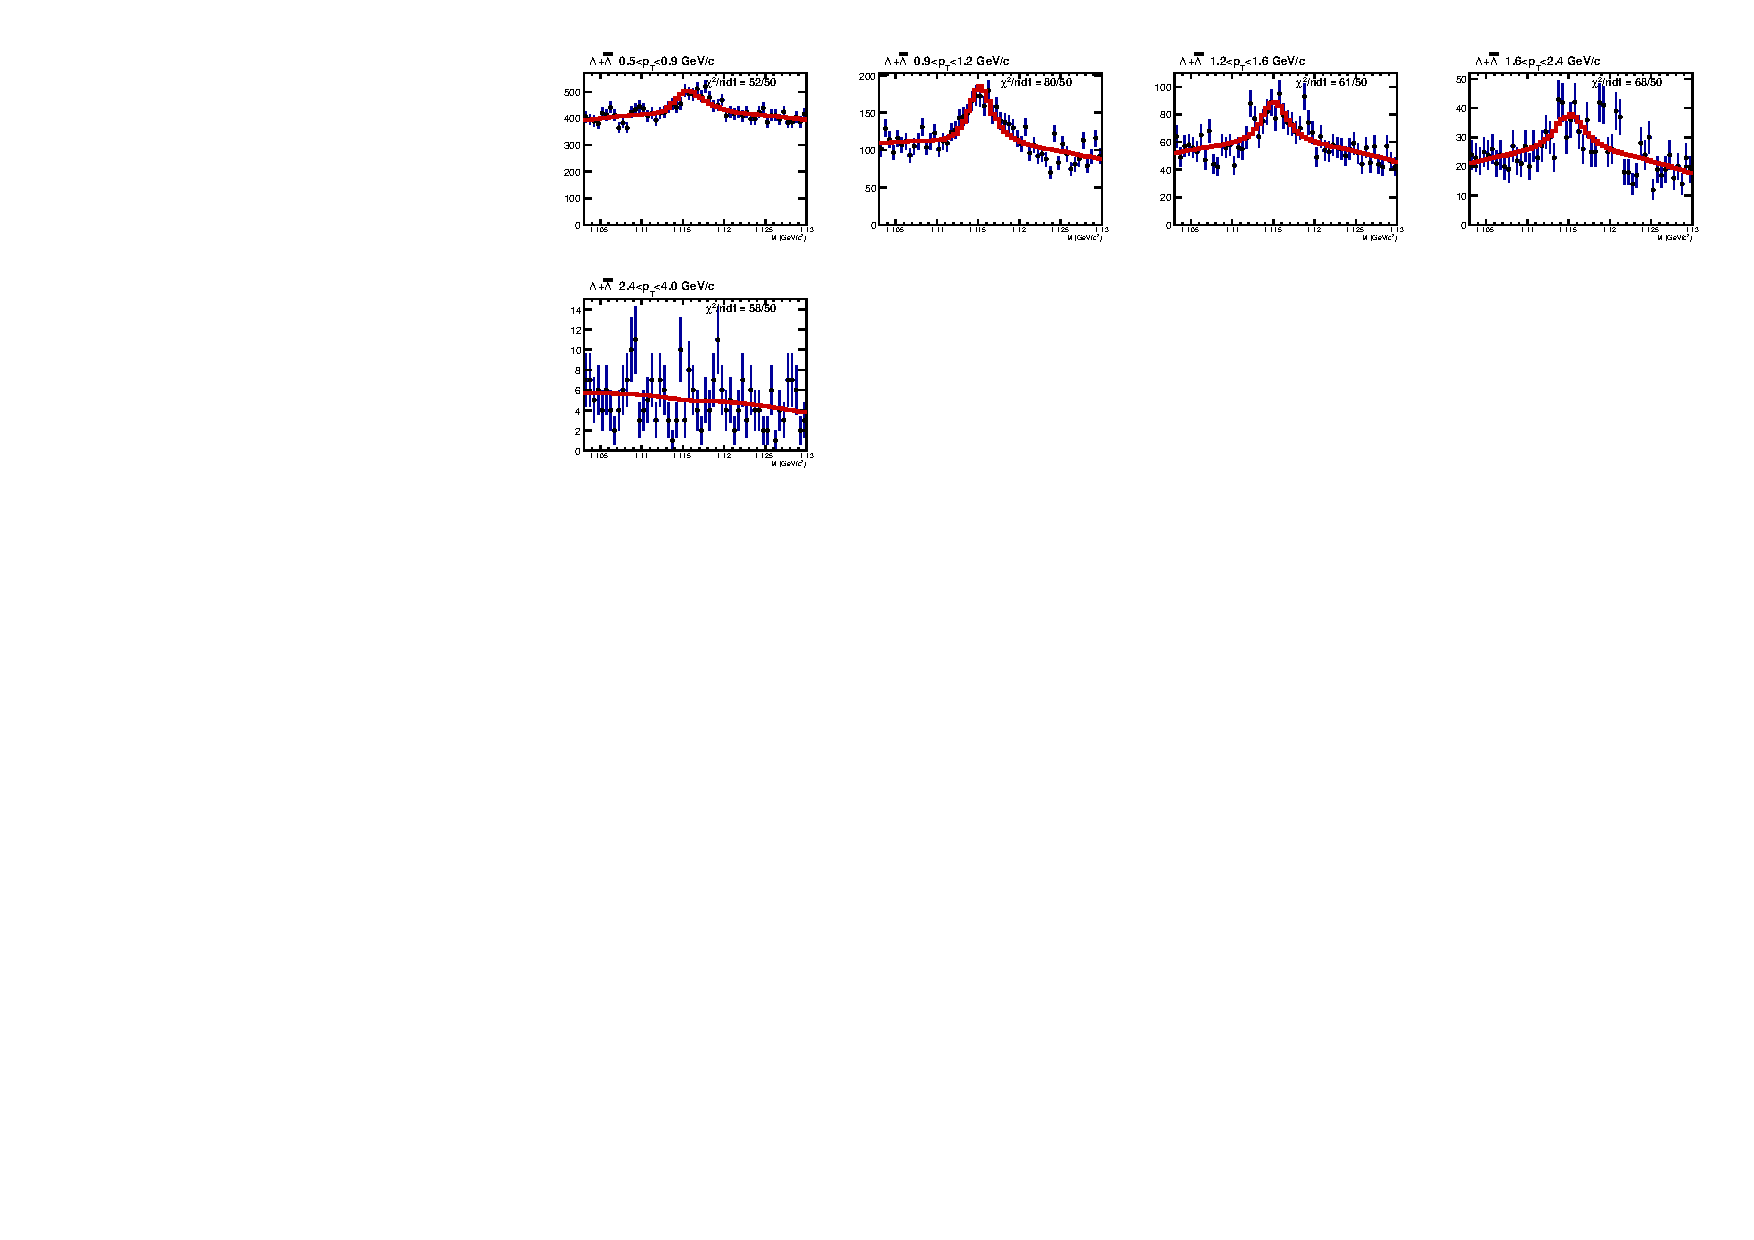
\includegraphics[width=\textwidth]{fig_mass_Lambda_B_raw}
\caption{As above, period B.}
\end{figure}
